%%% License: Creative Commons Attribution Share Alike 4.0 (see https://creativecommons.org/licenses/by-sa/4.0/)
%%% Slides are based heavily on earlier versions of this course taught by Jesper Rudiger.

\documentclass[english,10pt
,aspectratio=169
%,handout
%,notes
]{beamer}
%%% License: Creative Commons Attribution Share Alike 4.0 (see https://creativecommons.org/licenses/by-sa/4.0/)
%%% Slides are based heavily on earlier versions of this course taught by Jesper Rudiger and Peter Norman Sorensen.

\DeclareGraphicsExtensions{.eps, .pdf,.png,.jpg,.mps,}
\usetheme{reMedian}
\usepackage{parskip}
\makeatother

\renewcommand{\baselinestretch}{1.1} 

\usepackage{amsmath, amssymb, amsfonts, amsthm}
\usepackage{enumerate}
\usepackage{hyperref}
\usepackage{url}
\usepackage{bbm}
\usepackage{color}

\usepackage{tikz}
\usepackage{tikzscale}
\newcommand*\circled[1]{\tikz[baseline=(char.base)]{
		\node[shape=circle,draw, inner sep=-20pt] (char) {#1};}}
\usetikzlibrary{automata,positioning}
\usetikzlibrary{decorations.pathreplacing}
\usepackage{pgfplots}
\usepgfplotslibrary{fillbetween}
\usepackage{graphicx}

\usepackage{setspace}
%\thinmuskip=1mu
%\medmuskip=1mu 
%\thickmuskip=1mu 


\usecolortheme{default}
\usepackage{verbatim}
\usepackage[normalem]{ulem}

\usepackage{apptools}
\AtAppendix{
	\setbeamertemplate{frame numbering}[none]
}
\usepackage{natbib}


\usepackage{setspace}


\title{Financial Markets Microstructure \\ Lecture 1}

\subtitle{Introduction and institutions \\
Chapters 0 and 1 of FPR}

\author{Egor Starkov}

\date{K{\o}benhavns Universitet \\
	Spring 2021}



\begin{document}
\AtBeginSection[]{
\frame{
	\frametitle{This slide deck:}
	\tableofcontents[currentsection,currentsubsection]
}}
\frame[plain]{\titlepage}
\addtocounter{framenumber}{-1}


\begin{frame}
	Cameras on! (please?)
	
	for your sake as much as mine
\end{frame}


\section{Logistics}

\begin{frame}{Contact Information}
Lecturer: Egor Starkov
\begin{itemize}
	\item Contact: absalon or email (\href{mailto:egor.starkov@econ.ku.dk}{\texttt{egor.starkov@econ.ku.dk}})
	%\item Office: 26.1.13
	\item Office hours: by appointment (or after lectures)
\end{itemize}
\end{frame}


\begin{frame}{Schedule}
\begin{columns}
	\begin{column}{0.6\linewidth}
		2 hours of lectures once or twice a week
		\begin{itemize}
			\item \structure{Wednesdays 13.00-15.00} (weeks 6-21); %
			\item \structure{Fridays 10.00-12.00} (weeks 7,9,11,15,17,19).
			\item (That's 22 lectures when we are only supposed to have 21. May skip one or use for office hours/exercise class/...)
			\item on Zoom, until April 1 and/or further notice.
		\end{itemize}
	\end{column}
	\begin{column}{0.4\linewidth}
		\pause[1]
		\includegraphics<handout:0>[scale=0.14]{pics/schedule}
	\end{column}
\end{columns}
\end{frame}


\begin{frame}{Resources}
\begin{columns}
	\begin{column}{0.7\linewidth}
		{\setstretch{1.3}
		\begin{itemize}
			\item Get the book by Foucault, Pagano, and R{\"o}ell.
			\begin{itemize}
				\item We'll be using it a lot (incl. exercises).
				\item Will switch to research articles towards the end of the course.
			\end{itemize}
			\item Everything else (lectures, problem sets for exercise classes, etc.) is on \alert{Absalon} -- check regularly.
			% walkthrough of absalon (pages, calendar, syllabus, zoom)
			\item I will upload the \alert{slides} before the lectures for you to print out.%
			\begin{itemize}
				\item Those may contain omissions! % if i'm not lazy
			\end{itemize}
			\pause 
			\item \alert{Recordings} will be uploaded to absalon files
			\begin{itemize}
				\item \structure{Limited space} $\rightarrow$ deleted after 3-5 weeks
				\item \structure{GDPR} $\rightarrow$ you must delete the recordings after the course has concluded
				\item There is always a slight chance of some catastrophic failure (=no recording)
				\item \structure{Last year's lectures} are \href{https://www.youtube.com/playlist?list=PL4pUs4P_j1Wa2_P1lw44kFWWjKDTGUY7S}{\uline{on youtube}}.
			\end{itemize}
		\end{itemize}
		}
	\end{column}
	\begin{column}{0.3\linewidth}
		\pause[1]
		\includegraphics<handout:0>[scale=1]{pics/resources}
	\end{column}
\end{columns}
\end{frame}


\begin{frame}{Problem sets and Exam}
\begin{columns}
	\begin{column}{0.6\linewidth}
		{\setstretch{1.3}
			\begin{itemize}
				\item \alert{readings and exercises} after lectures (esp. in earlier part of the course)
				\begin{itemize}
					\item voluntary; will go through some in class
					\item readings not always immediately related to theory, but always related to the course
				\end{itemize}
				\item 2 problem sets (larger, cumulative, more open-ended?)
				\begin{itemize}
					\item Voluntary too. Take them as an opportunity to check your progress
				\end{itemize}
				\item \alert{final exam}: 12-hr take-home exam.
			\end{itemize}
		}
	\end{column}
	\begin{column}{0.4\linewidth}
		\pause[1]
		\includegraphics<handout:0>[scale=0.08]{pics/exam}
	\end{column}
\end{columns}
\end{frame}


\begin{frame}{Covid reality}
	\begin{columns}
		\begin{column}{0.6\linewidth}
			{\setstretch{1.3}
				\begin{itemize}
					\item Everything is online-only until further notice.
					\item It's difficult to make things work, but let's try.
					\pause
					\item \alert{Group work}!
					\begin{itemize}
						\item Organize into groups and work on homeworks together!
						\item Set up a weekly meeting time?
						\item Do ``viewing parties'' for lectures?
						\item Message me before EoD Friday if you are \alert{looking for a group} or group members.
					\end{itemize}
					\pause
					\item \structure{Group activities}
					\begin{itemize}
						\item I will try to organize more discussions in class.
					\end{itemize}
					\item Questions during class: just unmute and speak; I try to read chat but no promises; I will not see ``raised hands''.
				\end{itemize}
			}
		\end{column}
		\begin{column}{0.4\linewidth}
			\pause[1]
			\includegraphics<handout:0>[scale=0.27]{pics/covid}
		\end{column}
	\end{columns}
\end{frame}




\section{Why do we need financial markets?}

\begin{frame}{Why do we need markets?}
\begin{columns}
	\begin{column}{0.6\linewidth}
		\begin{enumerate}
			\item \alert{What} is a market?%
			\visible<handout:0|2->{
				\begin{itemize}
					\item Institution for property rights exchange
				\end{itemize}
			}
			\medskip
			\pause[1]
			\item \alert{Why} do we need markets?
			\pause[2]
			\visible<handout:0|3->{
				\begin{itemize}
					\item Want property rights to be allocated \structure{efficiently} in the society
					\item Smooth functioning of markets is essential for this
				\end{itemize}
			}
		\end{enumerate}
	\end{column}
	\begin{column}{0.4\linewidth}
		\pause[1]
		\includegraphics<handout:0>[scale=0.11]{pics/market}
	\end{column}
\end{columns}
\end{frame}


\begin{frame}{Why do we need Financial Markets?}
\begin{columns}
	\begin{column}{0.6\linewidth}
		\begin{itemize}
			\item \textbf{Financial markets}: markets for financial assets
			\item \textbf{Financial assets}: move wealth across time and contingencies: 
			\begin{itemize}
				\item Financial assets provide `contingent cash flows'
				\item Stocks, bonds, derivatives...
			\end{itemize}
			\pause
			\item \textbf{Purposes} of financial markets:
			\visible<handout:0>{
				\begin{itemize}
					\item Forum for trade in the stock (\alert{consolidation});
					\item Each trader can compare his private valuation against the current price (\alert{transparency});
					\item Guarantee of getting what is paid for (\alert{security})
				\end{itemize}
			}
			\item \textbf{Specifics} of financial markets:
			\begin{itemize}
				\item Usually organized in a specific way and heavily regulated.
				\item Feature to a lot of asymmetric information
			\end{itemize}
		\end{itemize}
	\end{column}
	\begin{column}{0.4\linewidth}
		\pause[1]
		\includegraphics<handout:0>[scale=0.17]{pics/exchange}
	\end{column}
\end{columns}
\end{frame}



\section{Types of financial markets}

\begin{frame}{Types of Financial Markets}
	\begin{itemize} 
		\item \textbf{Primary markets}: ``Allocate savings to investment''
		\begin{itemize}
			\item Issues of new assets (typically by investment bank)
		\end{itemize}
		\item \textbf{Secondary markets}: ``Reallocate investments over savers''
		\begin{itemize}
			\item Trade in existing assets on exchange
		\end{itemize}	
		\pause
		\item This course: focus on secondary markets 
		\begin{itemize}
			\item Stock and bond markets
			\item Derivative markets
			\item Currency (FX) markets
			\item Most insights will apply to commodity markets that deal in futures (oil, metals...) 
		\end{itemize}
	\end{itemize}
\end{frame}


\begin{frame}{Market Setups}
Two (three?) rough categories of market setups
\begin{enumerate}
	\item Decentralized ``markets''
	\item Dealer markets
	\item Order-driven markets
	\begin{itemize}
		\item Continuous
		\item Call
	\end{itemize}
\end{enumerate}
\end{frame}


\begin{frame}{Direct trading}
\begin{columns}
	\begin{column}{0.6\linewidth}
		\begin{itemize}
			\item Buyers and sellers could interact \structure{directly}.
			\item A useful benchmark, but not a very interesting case.
		\end{itemize}
	\end{column}
	\begin{column}{0.4\linewidth}
		\pause[1]
		\includegraphics<handout:0>[scale=0.27]{pics/ag_direct}
	\end{column}
\end{columns}
\end{frame}


\begin{frame}{Dealer Markets}
\begin{columns}
	\begin{column}{0.6\linewidth}
		\begin{itemize}
			%\item Unlike order-driven markets, prices are fixed by a dealer
			\item A \structure{dealer} quotes a bid and an ask price (valid up to certain number of shares)
			\item Bid-ask spread:
			\begin{itemize}
				\item Narrow to fend off competitors
				\item Wide to generate trading profits
			\end{itemize}
			%\item How competitive are the prices?
			%\item Dealer costs:
			%\begin{itemize}
			%	\item Transactions and operations costs
			%	\item Inventory costs
			%	\item Adverse selection costs
			%\end{itemize}
			\item Dealer exchanges: Nasdaq
		\end{itemize}
	\end{column}
	\begin{column}{0.4\linewidth}
		\pause[1]
		\includegraphics<handout:0>[scale=0.27]{pics/ag_dealer}
	\end{column}
\end{columns}
	
\end{frame}


\begin{frame}{Order-driven markets}
\begin{columns}
	\begin{column}{0.6\linewidth}
		\begin{itemize}
			\item Timing
			\begin{enumerate}
				\item Orders are submitted
				\item Trades are arranged
			\end{enumerate}
			\item The markets can vary in different ways
			\begin{itemize}
				\item Frequency of trading: how often?
				\item Order precedence: price/time/public
				\item Pricing rule: uniform/discriminatory price, determined from orders/taken from other exchange
				\item Opening/closing: are there any special trading rules?
			\end{itemize}
		\end{itemize}
	\end{column}
	\begin{column}{0.4\linewidth}
		\pause[1]
		\includegraphics<handout:0>[scale=0.27]{pics/ag_exch}
	\end{column}
\end{columns}

\end{frame}


\begin{frame}{Order types}
\begin{itemize}
	\item There's a tremendous amount of different order types. We focus on two main ones:
	\item \textbf{Market order} specifies quantity: ``buy 500 shares at best available price''.
	\item \textbf{Limit order} specifies a quantity and a price: ``will buy 500 shares at below price 40''
	\item Trades occur either through 
	\begin{enumerate}
		\item a limit order 'match' (somebody posts a bid price above the lowest ask price), or
		\item through market orders
	\end{enumerate}
\end{itemize}
\end{frame}


\begin{frame}{Order-driven markets: Continuous auctions}
\begin{itemize}
	\item LOs together compose a \structure{Limit Order Book}.
	\begin{itemize}
		\item Any given LO can be \textbf{marketable} or not.
		\item A marketable LO is expected to execute immediately given other orders in the LOB.
	\end{itemize}
	\item Traders can choose orders best for them:
	\begin{itemize}
		\item Patient traders are more passive: use limit orders (fill LOB)
		\item Impatient traders are more aggressive: use market orders (deplete LOB)
	\end{itemize}
	\item \alert{Discriminatory price}: depends on how your order is matched
	\item Continuous LOB exchanges: NYSE (both electronic and `outcry'), LSE, BATS, Euronext
\end{itemize}
\end{frame}


\begin{frame}{Order-driven markets: Call (batch) auctions}
\begin{itemize}
	\item Orders are collected (in a `batch') and cleared at a certain frequency
	\item The price is chosen so as to maximize the number of executed orders
	\item \alert{Uniform price}: all orders in a batch trades at same price
	\item In theory,  very good efficiency properties: all profitable trades are carried out
	\item But... slower than the continuous market
	\item Call auction exchanges: most of the major exchanges (e.g. Nasdaq, LSE, Euronext) operate call auctions together with other trading methods
\end{itemize}
\end{frame}


\begin{frame}{Exchange versus over-the-counter}
\textbf{Exchange trading}
\begin{itemize}
	\item Organized exchange venues (NYSE, NASDAQ, LSE, ...)
	\item Generally offer a lot of services
	\begin{itemize}
		\item Liquidity and stability through \textit{specialists/market makers}
		\item Clearing and settlement
		\item Transparency
	\end{itemize}
\end{itemize}
\textbf{Over-the-counter (OTC) trading}
\begin{itemize}
	\item Off-exchange venues
	\begin{itemize}
		\item Use quotation systems to match dealers and traders
		\item However, no guarantee of liquidity (no specialists)...
		\item ...nor transparency: may not publish trade information
	\end{itemize}
\end{itemize}
\textbf{Dark liquidity}: Liquidity in `private exchanges' (not public)
%NOTE: Amazon is like an exchange (provides basic products in all categories); eBay/FB is OTC (only matches buyers and sellers);
%NOTE: Difference between OTC and Dark is whether offers/quotes are public or not (although DARK a subset of OTC?)
\end{frame}


\begin{frame}{Other dimensions}
	\begin{itemize}
		\item Many other aspects in which markets can differ:
		\begin{itemize}
			\item Transparency about current orders
			\item Transparency about past trades
			\item Fragmentation
			\item Listing requirements
			\item ...
		\end{itemize}
		\item Who benefits from markets being organized in a particular way? Who loses? 
	\end{itemize}
\end{frame}


%\begin{frame}{Comparison}
%	What to consider when comparing these markets?
%	\begin{itemize}
%		\item \textbf{Welfare planner}: Competition - efficiency 
%		\item \textbf{Trader}: Liquidity - transparency - information
%	\end{itemize}
%\end{frame}


\section{Types of agents in financial markets}

\begin{frame}{Players}
\begin{columns}
	\begin{column}{0.4\linewidth}
		\begin{itemize}
			\item \textbf{Traders/investors}: the end-``consumers'' or suppliers of the asset
			\item \textbf{Brokers}: the intermediaries who relay investors' orders to the market (investment banks)
			\item \textbf{Dealers/market-makers}: match orders from different sides of the market
		\end{itemize}
	\end{column}
	\begin{column}{0.6\linewidth}
		\pause[1]
		\includegraphics<handout:0>[scale=0.23]{pics/ag_brokers}
	\end{column}
\end{columns}
\end{frame}


\begin{frame}{Types of traders}
Traders can be classified:
\begin{itemize}
	\item \structure{Retail investors} vs \structure{institutional investors}
	\begin{itemize}
		\item Retail: regular people, individuals with money.
		\item Institutional: pension funds, mutual funds, hedge funds, private equity funds...
	\end{itemize}
	\item \alert{Informed} vs \alert{uninformed} investors
	\begin{itemize}
		\item Retail investors and pension funds usually have little ``private information''.
		\item Hedge funds and short-selling funds have good analytics and can react fast.
		\item ``Private information''$\neq$``insider information''! Insider trading is banned in most jurisdictions.
	\end{itemize}
\end{itemize}
\end{frame}






\section{Next on...}

\begin{frame}{Motivating questions}
	\begin{enumerate}
		\item How are market prices created? How are they influenced by traders?
		\item How should traders act on their information?
		\item Do the market rules matter? And which rules are good for whom?
		\item How do we measure if markets are working well?
		%\begin{itemize}
		%	\item Liquidity/depth (a lot more on that later)
		%	\item Volume
		%	\item Efficiency
		%	\item Stability
		%\end{itemize}
	\end{enumerate}
\end{frame}


\begin{frame}{Course overview}
	\begin{itemize}
		\item Institutional details, policy issues, applications (ch.1, 6-10, articles)
		\item Theories to understand and to analyze policy (ch.3-4, 6-10, articles)
		\item Some empirical issues (ch.2, 5, articles)
	\end{itemize}
	
	\textbf{Prerequisites}: Finance, micro, games, (math)
	
	\textbf{Disclaimer}: We focus on `rational' models in this course.
	Behavioral finance is a complementary and exciting topic. See
	Alexander Sebald's course.
\end{frame}


\begin{frame}{For next class}
\begin{enumerate}
	%\item Find bid and ask prices for Facebook shares and for Microsoft. Which stock exchange do they come from? 
	\item Match into groups / message me if you are looking for a group or group members.
	\item Read the article about GameStop (on Absalon) and any follow-ups you can (be bothered to) find. Discuss in your newly formed groups:
	\begin{itemize}
		\item What kind of traders are involved on both sides? Based on that fact: why has this story made the news?
		\item Sentiment aside, would now be a good time to buy GameStop stock? Why/why not?
		\item Robinhood (trading app) halted trading in GameStop stocks at some point. Is there a scope for some regulatory intervention to prevent this kind of exclusion of retail traders?
	\end{itemize} 
	\item Do exercises 1-3 after Chapter 1 (pages 44-45) in the textbook
\end{enumerate}
\end{frame}

\end{document} 














%\begin{frame}{Many things happening now}
%	\begin{figure}
%		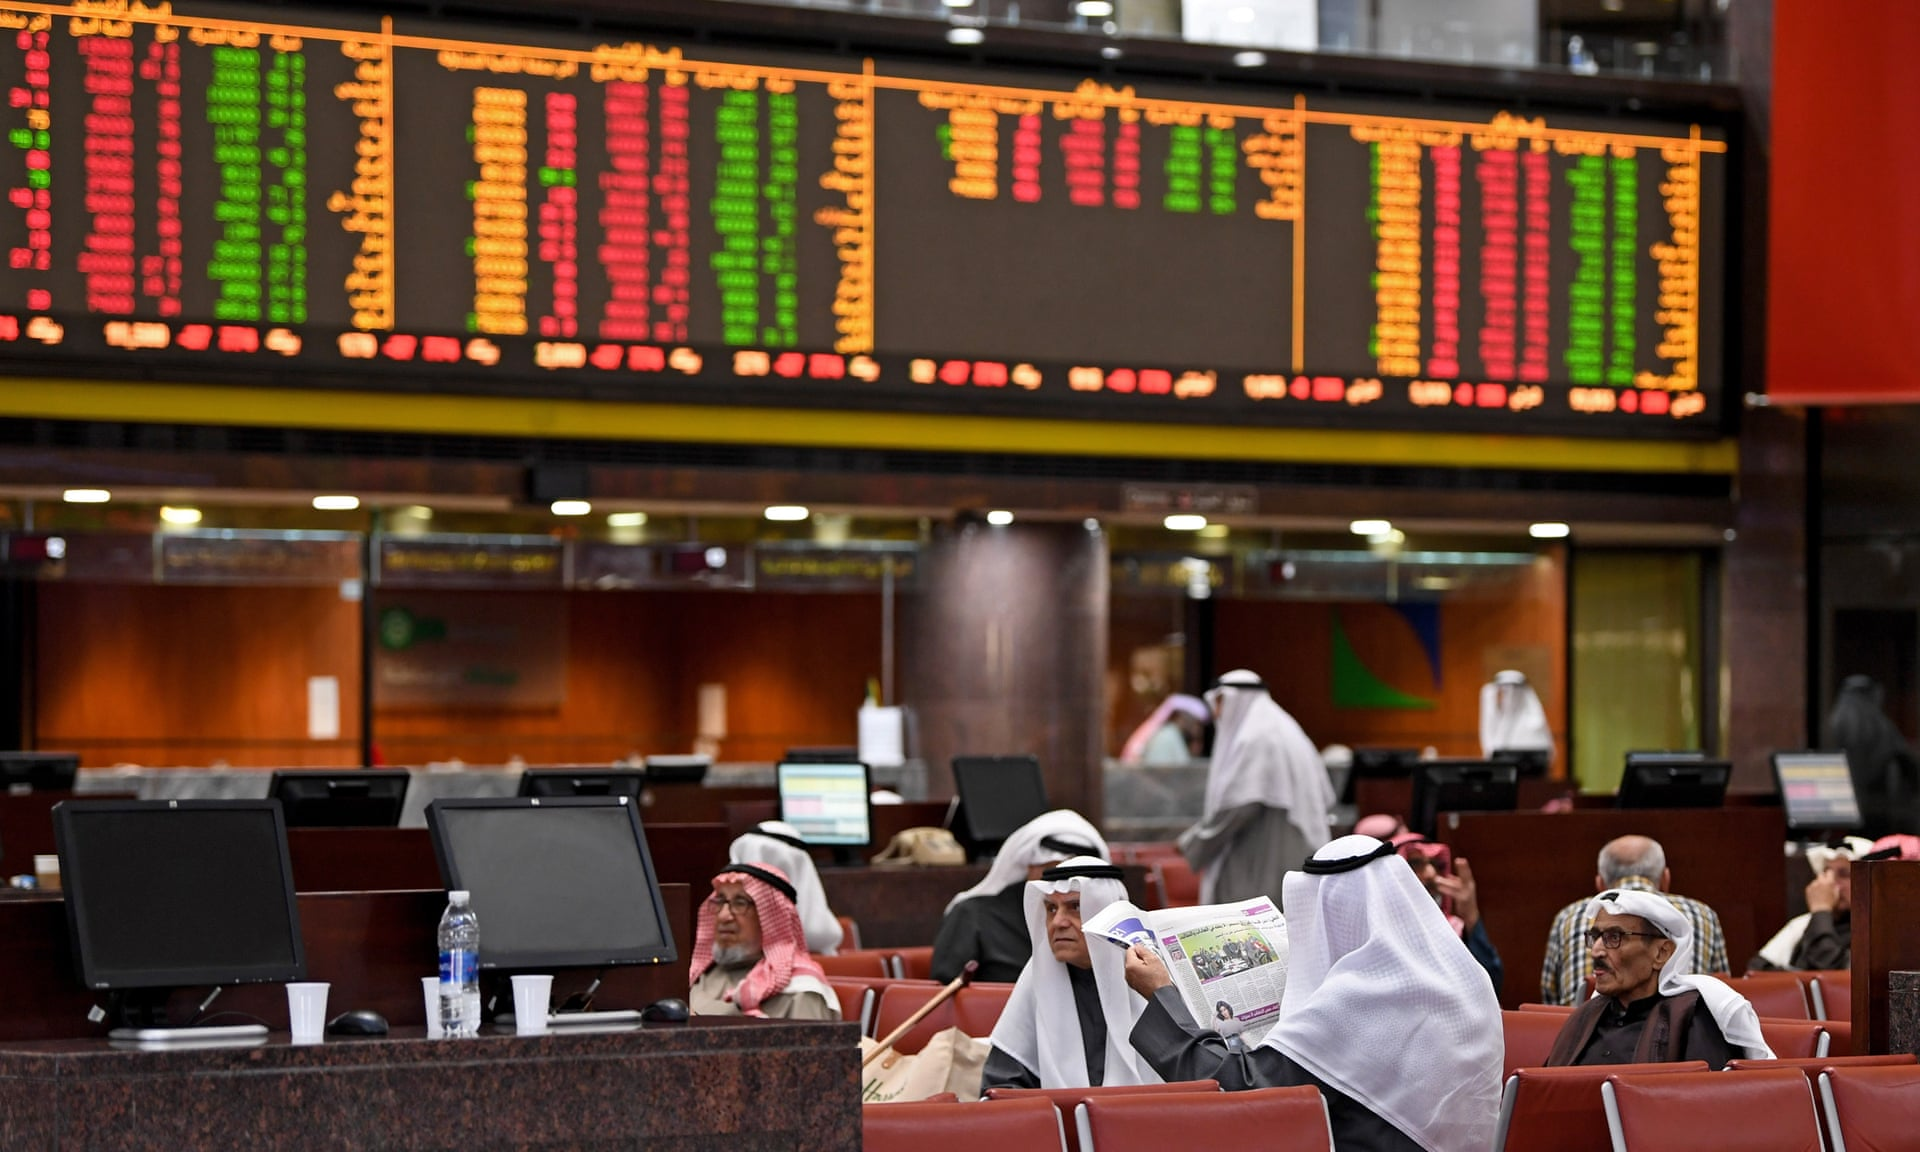
\includegraphics[width=.78\linewidth]{pics/markets2020}
%		\caption{The Guardian, January 6}
%		%NOTE: photo: Kuwait exchange trading floor.
%		%NOTE: Stock exchanges dropped on Jan 7 after Trump's attack on Iran and the retaliation that followed. Oil prices surged. A rebound followed after both sides announced easing out.
%	\end{figure}
%\end{frame}


%\begin{frame}{Main goals}
%\begin{enumerate}
%	\item Explain, discuss and interpret concepts and results from textbook and articles
%	\item Derive and analyze results in models
%	\item Discuss possible applications of theoretical concepts to problems
%\end{enumerate}
%Method: Carefully read texts, combine with facts, discuss, try problems
%\pause
%
%\textbf{Disclaimer}: We focus on `rational' models in this course.
%Behavioral finance is a complementary and exciting topic. See
%Alexander Sebald's course.
%\end{frame}



%\section{Core concepts}

\begin{frame}{Today's plan}
	\tableofcontents[currentsection]
\end{frame}

\begin{frame}{Trade and Prices}
	\begin{itemize}
		\item Price theory is fundamental to economics
		\begin{itemize}
			\item Law of one price; no arbitrage
		\end{itemize}
		\item In financial markets: often a \textit{bid} and an \textit{ask} price. The difference between the two is called the `\textbf{bid-ask spread}'
		\begin{itemize}
			\item We will spend time analyzing what drives this spread
		\end{itemize}
		%	\item Important question: How are prices formed?
		%	\begin{itemize}
		%		\item Shed light on the invisible hand
		%		%\item Difference to standard market theory: assume that agents are strategic ($\rightarrow$ game theory) 
		%	\end{itemize}
		%\item Do markets result in efficient allocations?
	\end{itemize}
\end{frame}


\begin{frame}
	\centering
	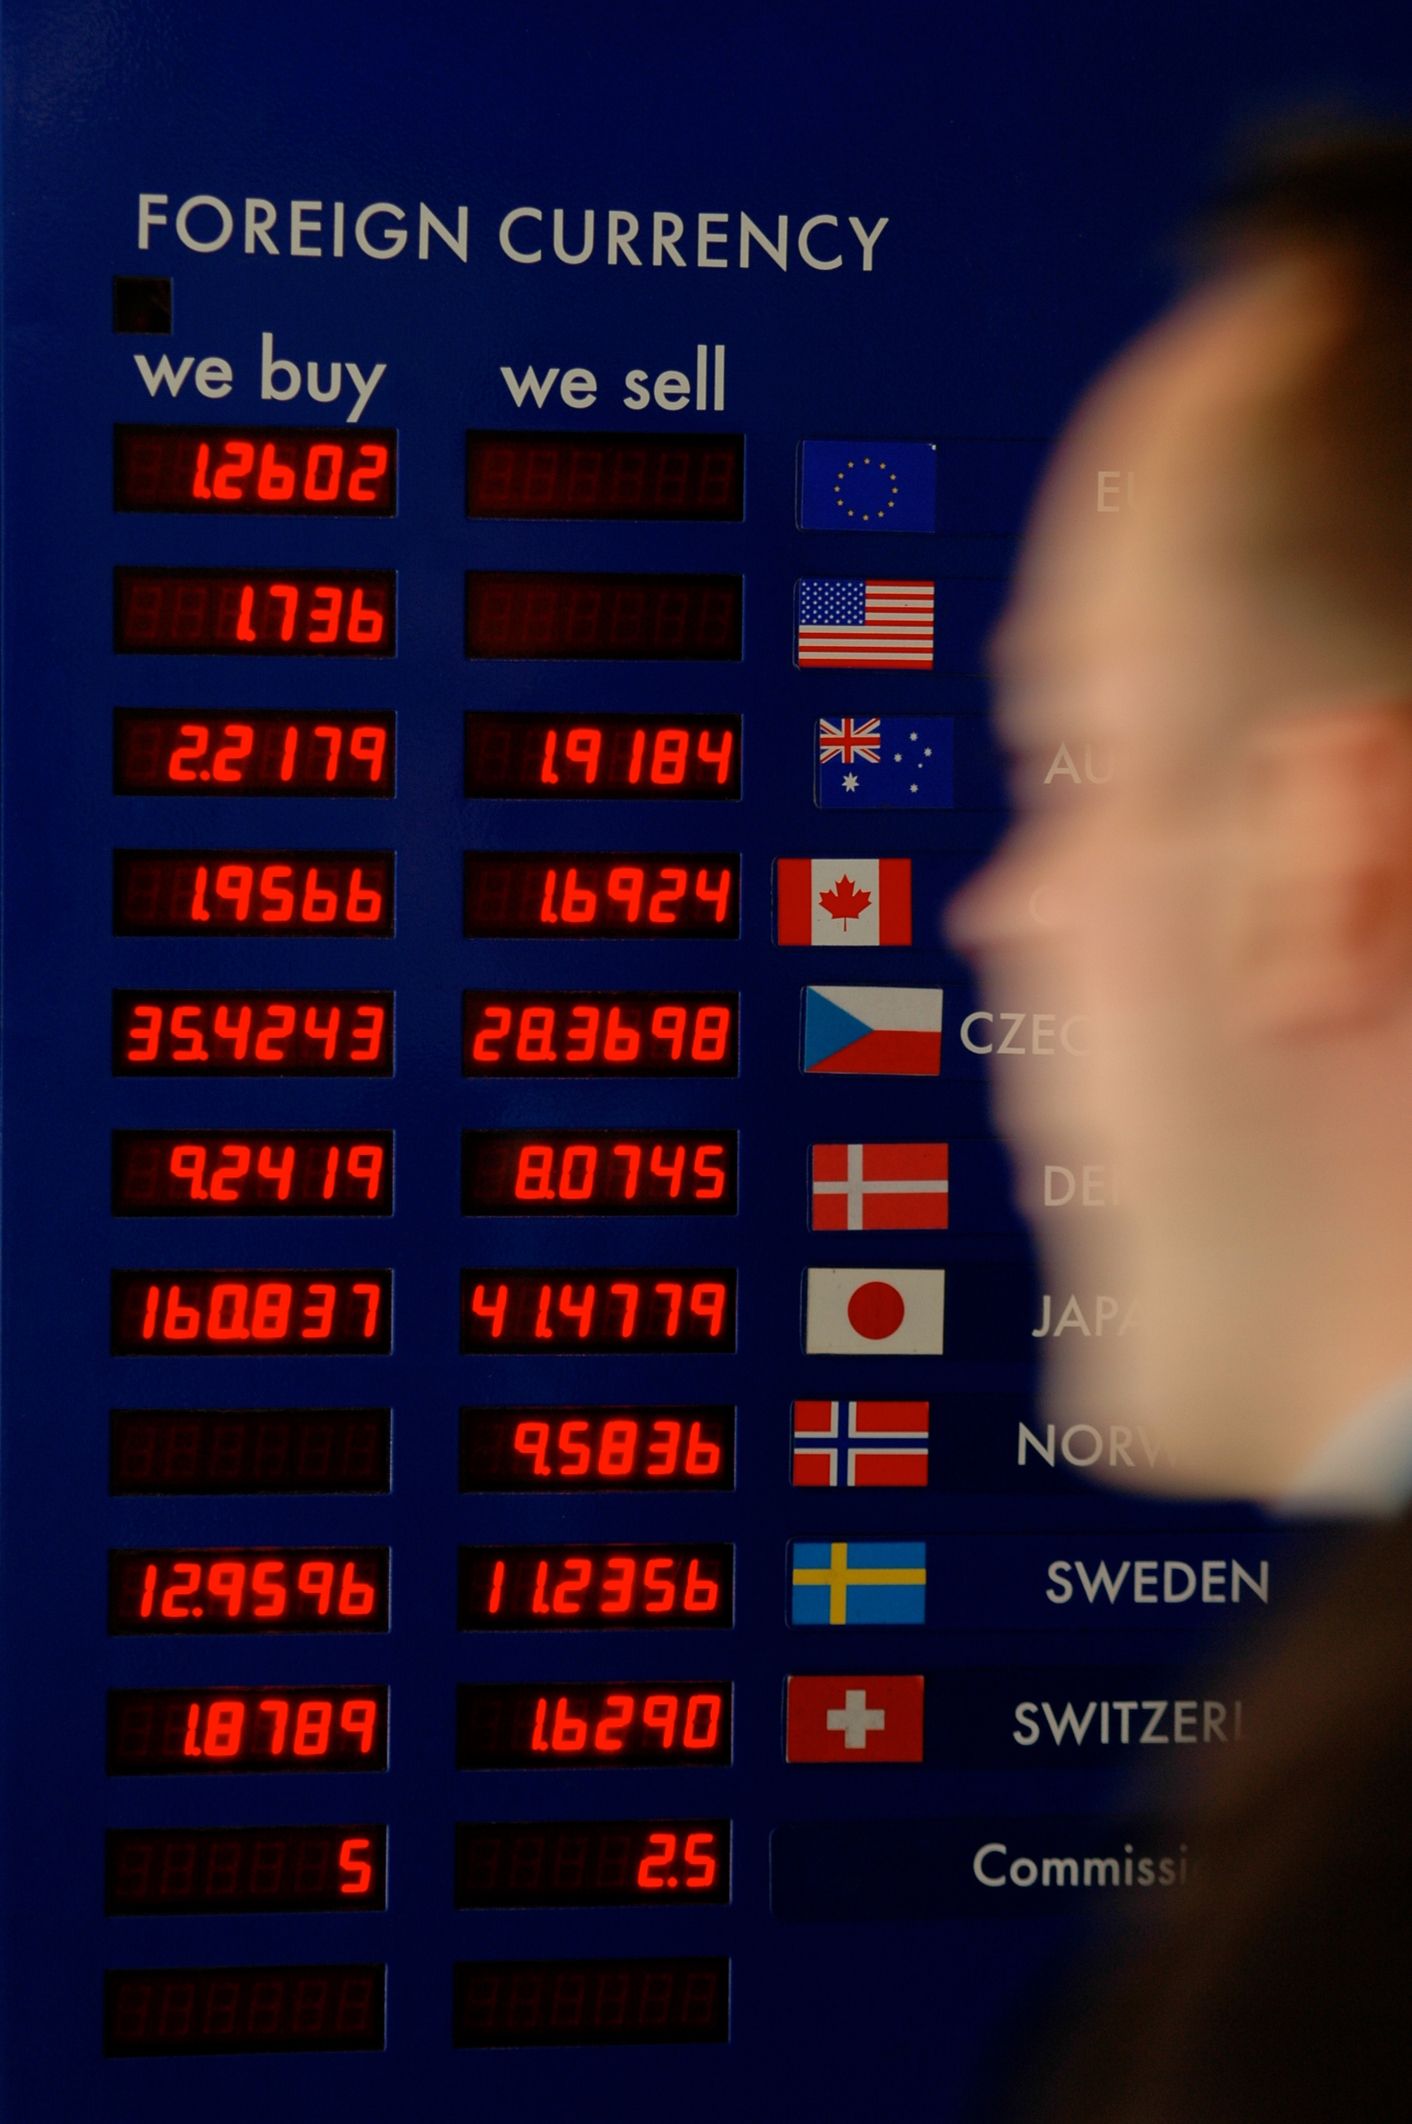
\includegraphics[width=.3\paperwidth]{pics/Image_XRates}
\end{frame}


\begin{frame}
	\centering
	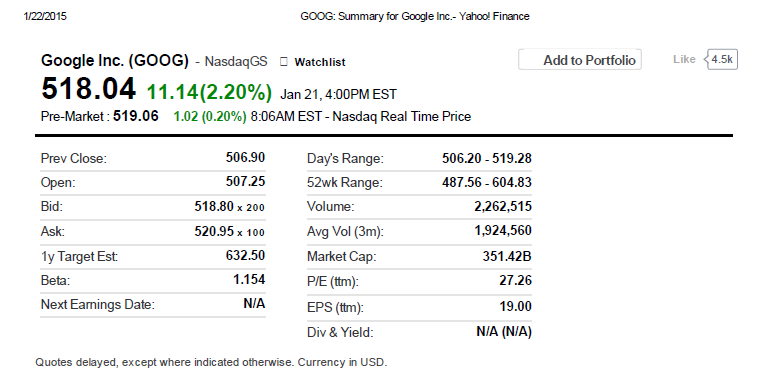
\includegraphics[width=1\linewidth]{pics/StockSummary_Google}
\end{frame}


\begin{frame}[label=main4]{Fundamental Value}
	\begin{itemize}
		\item Consider Google Stock
		\item What is the \textbf{fundamental value} of its stock? Where does it come from?
		\begin{enumerate}
			\item R+D
			\item Governance
			\item Marketing
			\item Competition
			\item ...
		\end{enumerate}
		\item In this course: take the `fundamental value' as given and analyze how it translates into prices
		
		\item \textbf{Price discovery}: how much information about the fundamental value can be extracted from market prices?
		
		\hyperlink{quote}{\beamerbutton{Quote}}
	\end{itemize}
\end{frame}


\begin{frame}{Market Liquidity}
	\begin{itemize}
		\item So far, you have been used to analyzing (long-run) equilibrium allocations and prices
		\item In practice, prices adjust to temporary imbalances
		\begin{itemize}
			\item Not everyone who wants to trade in a given asset is present in the market at the same time
			\item Example: too many sellers $\rightarrow$ prices lower in short run
			\item Example: costly to execute large order quickly
		\end{itemize}
		\pause
		\item These effects are related to the \textbf{liquidity} of the asset
		\begin{itemize}
			\item Wikipedia: `market liquidity' is a market's ability to facilitate an asset being sold quickly without having to reduce its price very much
			\item Easy to sell a Google stock (many potential buyers), but maybe hard for a stock of a small Danish company
		\end{itemize}
		\item We will develop measures of liquidity in this course
		\item More liquid assets may be more valuable
	\end{itemize}
\end{frame}


\begin{frame}{Market depth}
	\begin{itemize}
		\item Prices are not always immediately available, even at an exchange
		\begin{itemize}
			\item You may observe previous trading prices, but nothing assures that future trading prices will be the same
			\item You may observe quotes from sellers/buyers, but quotes are normally only valid for a specific amount of stocks
		\end{itemize}
		\item A useful concept is \textbf{market depth}: it measures how big an order is required to change the price of an asset by, say, 10 cents
	\end{itemize}
\end{frame}


%\begin{frame}{Finally... The Big Issue}
%\begin{itemize}
%	\item Since this is a course on financial markets, we will also try to speak (a bit) about recent big events.
%	For instance...
%	
%	\begin{minipage}{.4\textwidth}
%		\begin{figure}
%		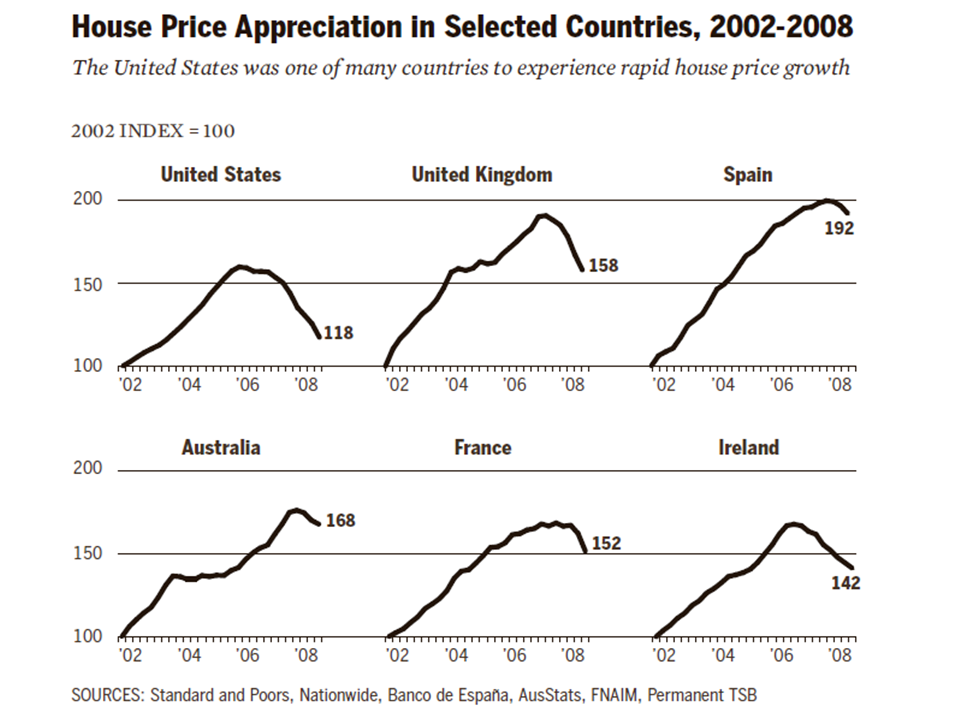
\includegraphics[width=1\linewidth]{pics/Graph_HousePrices}
%		\caption{Housing bubble}
%		\end{figure}
%	\end{minipage}
%	\quad
%	\begin{minipage}{.4\textwidth}
%		\begin{figure}
%		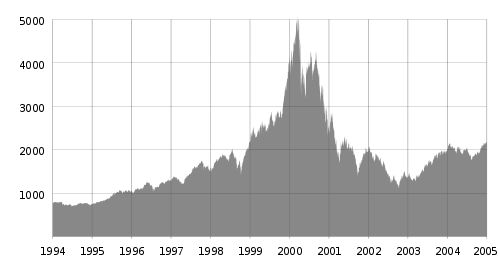
\includegraphics[width=1.3\linewidth]{pics/Graph_Nasdaq}
%		\caption{Tech bubble (Nasdaq index)}
%		\end{figure}
%	\end{minipage}
%	\item The last lectures of the course will be about this
%\end{itemize}
%\end{frame}




%\begin{frame}{Asset Markets}
%\begin{itemize}
%	%TODO: cut this slide?
%	\item \textbf{Markets}: facilitate trade between investors and savers
%	\item \textbf{Speculators}: interact with markets
%	\item \textbf{Intermediation}: done by dealers/brokers or automated systems
%	\item \textbf{Matching}: thus, the market matches buyers with sellers - important to attract both types of traders
%\end{itemize}
%\end{frame}



\begin{frame}{Regulation}
	Market rules and government regulation:
	
	\textbf{Goals:}
	\begin{itemize}
		\item Protection against insider traders, level the information flow
		\item Stabilize the market, for instance halts and short-sale bans
		\item More generally, select optimal trading structure for each asset type
	\end{itemize}
	\textbf{Methods:}
	\begin{itemize}
		\item Require routing of orders between markets
		\item Transactions tax
		\item Margin requirements
		\item Policies on algorithmic, high-frequent trading
	\end{itemize}
\end{frame}


\begin{frame}{Competition}
	\begin{itemize}
		\item Network externalities in trading may favor a single market place (natural monopoly)
		\item Competition may improve the terms offered to traders
		\begin{itemize}
			\item Should regulators require price transparency?
			\item Order routing
			\item Foster competitive market making?
		\end{itemize}
	\end{itemize}
\end{frame}


\begin{frame}{Volumes of trade}
	\begin{figure}
		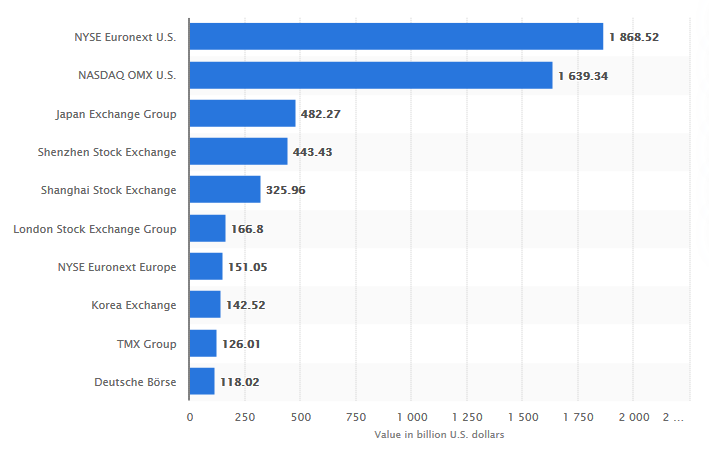
\includegraphics[width=.75\paperwidth]{pics/volumes2018}
	\end{figure}
	Largest stock exchanges worldwide in 2018, by value of electronic order book share trading, in billion USD (Statista)
\end{frame}